\section{CarryBotsの開発}
本章では,製作したロボットの概要について述べる.

\subsection{ロボットの概要}
上下のロボット間の摩擦力についてモデリングを行い,製作したロボット``CarryBot''を\reffig{carrybot}に示す.
本研究では他のロボットに乗り上げることを実現する機構として,ラックレール・ピニオン車輪構造を用いた.
さらに,\reffig{bottom}に示すようにピニオン車輪の歯先に滑りにくい軟質樹脂製パッドをつけ,車輪のグリップを高める.
そして,ロボットが物体の姿勢を検知するためのセンサとして,\reffig{diagonal}に示すようにリミットスイッチを採用した.
使用するモータは一つのみで,ギアを通じて車軸へ動力を伝達する.

\begin{figure}[tb]
  \begin{minipage}{\hsize}
  \centering
  \includegraphics[width=\columnwidth]{figures/carrybot-diagonal.pdf}
  \subcaption{Diagonal view}
  \label{fig:diagonal}
 \end{minipage}\\
 \begin{minipage}{\hsize}
  \centering
  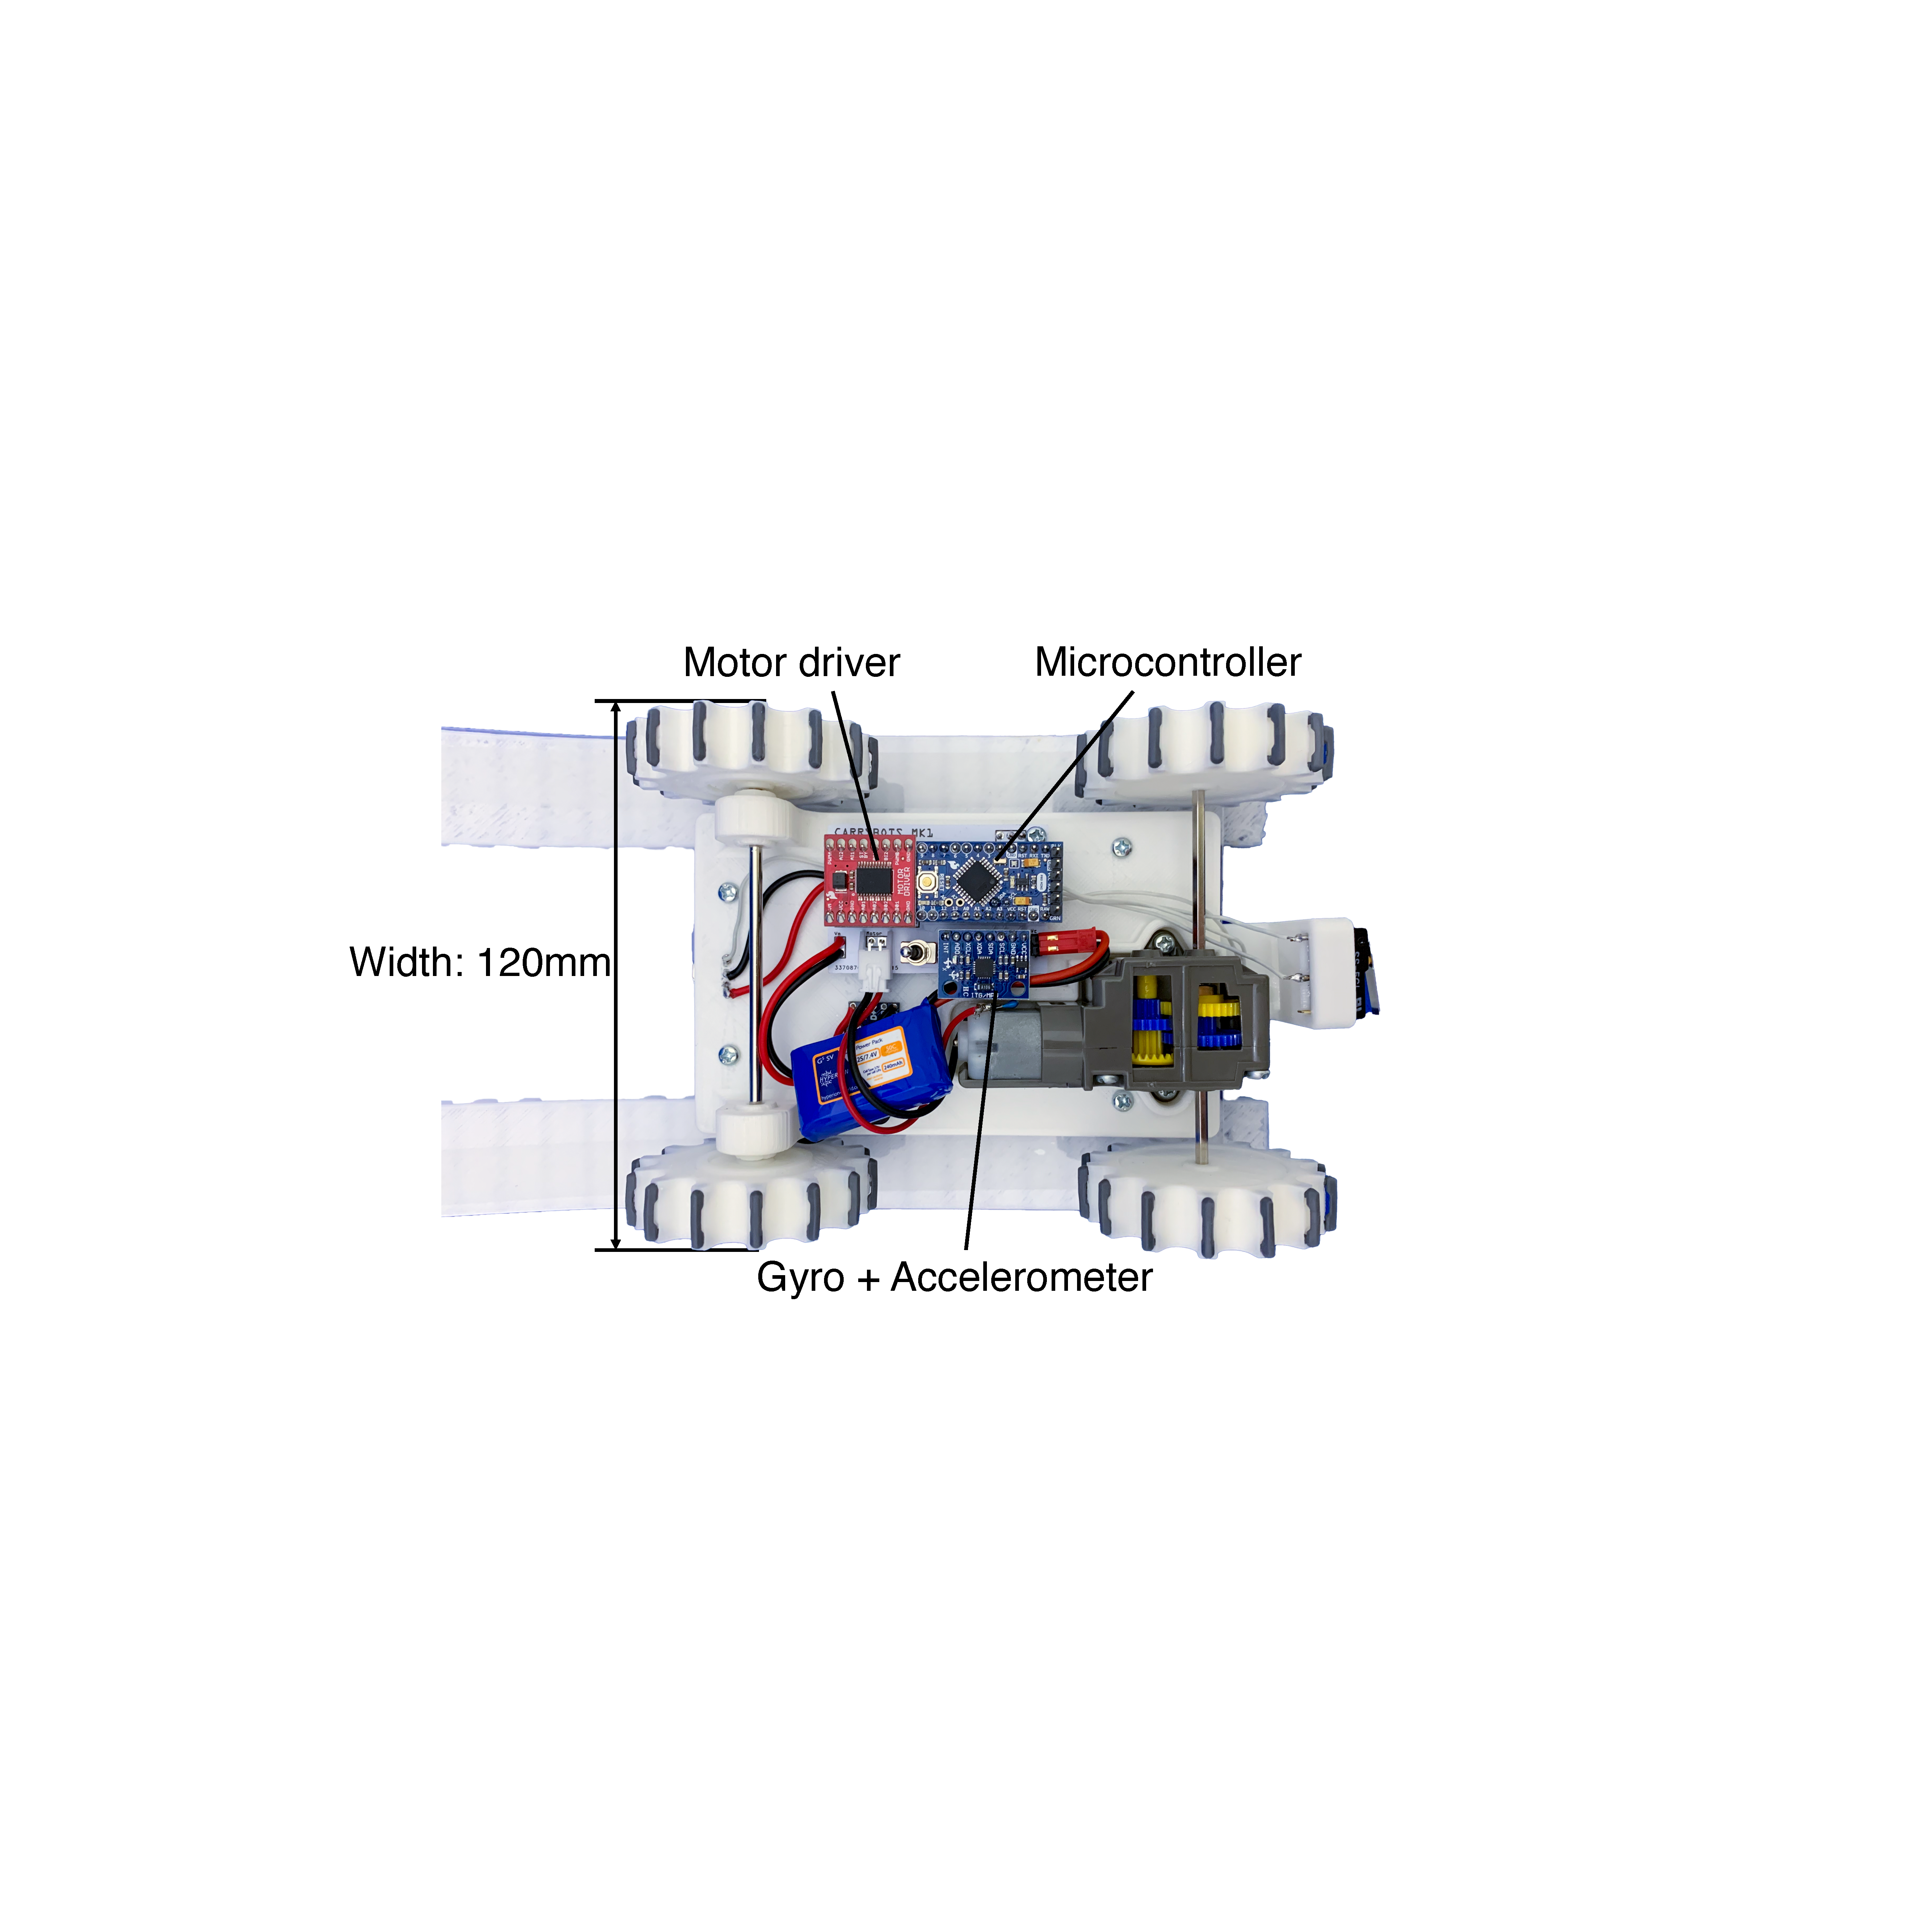
\includegraphics[width=\columnwidth]{figures/carrybot-bottom.pdf}
  \subcaption{Bottom view}
  \label{fig:bottom}
 \end{minipage}
 \caption{Mechanical structure of CarryBot}
 \label{fig:carrybot}
\end{figure}
